\documentclass[a4paper,12pt]{report}

\usepackage{alltt, fancyvrb, url}
\usepackage{graphicx}
\usepackage[utf8]{inputenc}
\usepackage{float}
\usepackage{hyperref}

% Questo commentalo se vuoi scrivere in inglese.
\usepackage[italian]{babel}

\usepackage[italian]{cleveref}

\title{Relazione per\\``IOT Assignment 2''}

\author{Andrea Zavatta - Lorenzo Tosi - Luca Pasini}
\date{\today}

\begin{document}

\maketitle

\tableofcontents

\newpage
\chapter{Analisi e Architettura}
\par
Abbiamo sviluppato questo progetto mediante un'architettura task based. Il sistema è diviso in Tasks, che eseguono ognuna i propri compiti. Ogni task ha un proprio periodo e un proprio workflow. L'esecuzione dei Tasks è controllata dallo scheduler.

\subsection{Task}
\par
Task.h è una classe astratta i cui metodi sono tutti implementati eccetto per il metodo tick, importante poiché definisce l'azione vera e propria dei singoli tasks e quindi dovrà essere implementato dalle classi che estendono questa classe astratta.
Ogni task può essere attivo o disattivo (di default sono tutti disattivi). Internamente il singolo task possiede un metodo che ne definisce il periodo (ovvero ogni quanto deve essere avviato), un metodo che controlla se l'esecuzione è terminata e un metodo che lo attiva o disattiva.

\subsection{Scheduler}
\par
Lo scheduler è una classe che ha 2 obiettivi: raggruppare tutti i task ed eseguirli. La prima funzionalità sfrutta la presenza di un array di task interno all'oggetto e utilizza un metodo di aggiunta di questi ultimi alla lista. La seconda funzionalità utilizza un metodo che controlla se i task sono attivi e, se lo sono, verifica se hanno finito la loro esecuzione. Se entrambi i controlli sono soddisfatti, allora lo scheduler fa eseguire l'azione al task; se invece almeno uno delle due condizioni non è soddisfatta, l'esecuzione di quel task specifico non avviene. Lo scheduler manda in esecuzione i task ogni intervallo di tempo, e quindi necessita che, alla creazione dell'oggetto, venga specificato il periodo.

\subsection{Stati}
\begin{figure}[H]
    \centering
    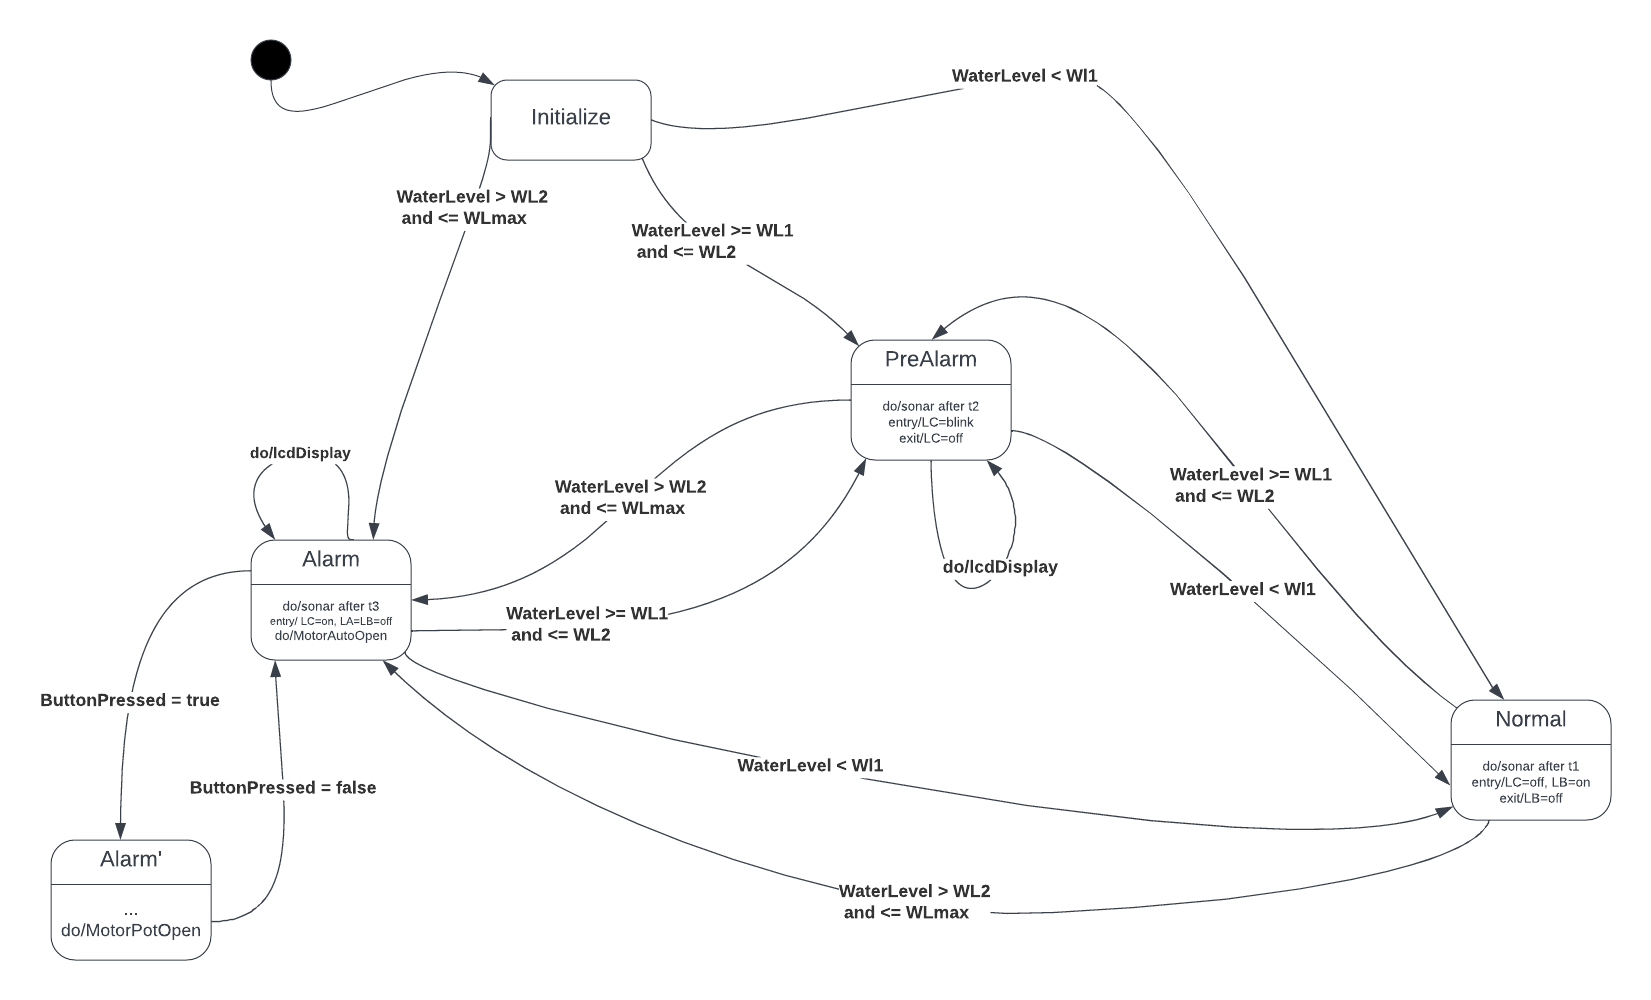
\includegraphics[width=13cm]{diagramma stati.png}
    \caption{rappresentazione uml degli stati generali}
\end{figure}

Il nostro sistema si basa su tre stati principali: normal, pre-alarm e alarm. Lo stato normal si presenta quando il livello dell'acqua (la distanza tra il sonar e un oggetto) si trova sopra la soglia di 0.50 metri; lo stato pre-alarm scatta quando questa soglia viene superata ma rimanendo sotto il limite di 0.30 metri. Infine, lo stato di allarme si verifica quando il livello dell'acqua è inferiore ai 0.30 metri di distanza. 
Per le specifiche elettroniche si fa riferimento alla traccia fornita dal docente.
Per trasformare le specifiche richieste in codice abbiamo deciso di sviluppare i seguenti task:
\begin{itemize}
    \item lcdTask
    \item ledTask
    \item lightSystemTask
    \item situationTask
    \item buttonTask
\end{itemize}
\begin{figure}[H]
    \centering
    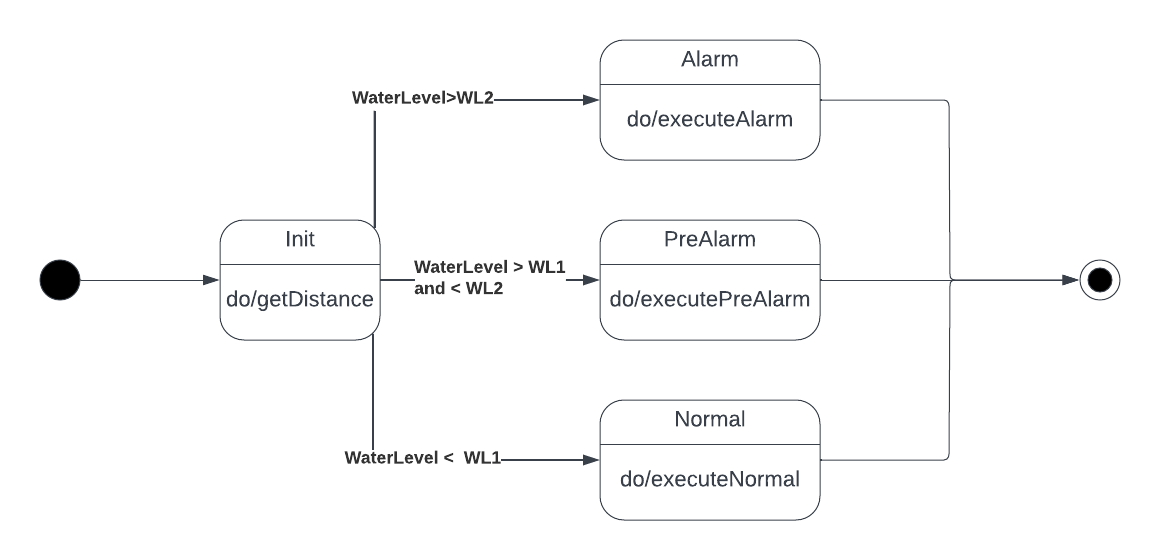
\includegraphics[width=13cm]{Blank diagram.png}
    \caption{rappresentazione uml del situationTask}
\end{figure}
\par
Il task più importante è situationTask, che gestisce il controllo del livello dell'acqua ottenuto grazie al sonar; il programma dunque si ritrova in uno dei 3 stati. È anche responsabile di chiamare il metodo che attiva o disattiva altri task. Internamente possiede quindi un riferimento all’oggetto del sonar, del motore e del potenziometro e alle task lcdTask e ledTask. Visto che la rilevazione del livello dell’acqua è gestita in questa task e deve essere eseguita in tempi diversi a seconda del livello dell’acqua, questo task è in grado di cambiare il proprio tempo di esecuzione. Infine, questa task possiede anche un array di listeners, ovvero task più complesse che stanno in ascolto dei cambiamenti e che, ogni volta che gli arriva la notifica, modificano il proprio comportamento in autonomia.

\begin{figure}[H]
    \centering
    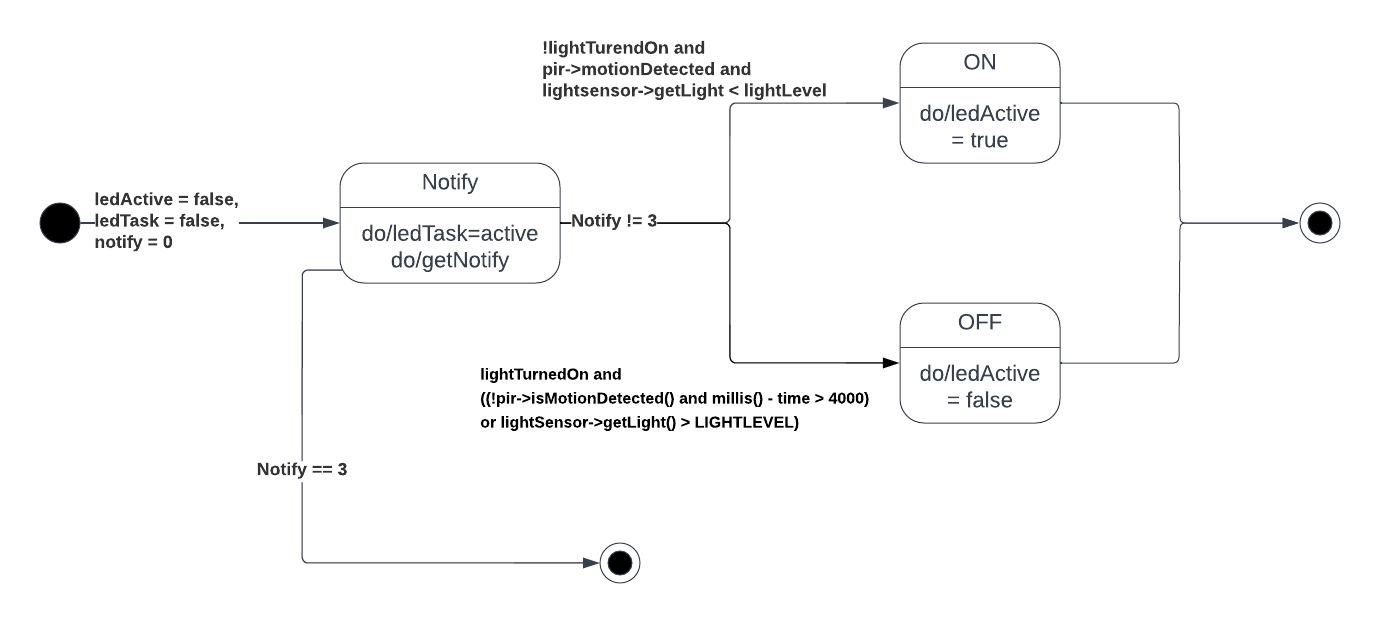
\includegraphics[width=13cm]{lightsystem.png}
    \caption{Rappresentazione uml del LightSystemTask}
\end{figure}

\par
La seconda task importante è la lightSystemTask, che gestisce il sistema di illuminazione del ponte. Internamente possiede un riferimento al pir, al sensore di luce e ad una ledTask. Questa task, attraverso il livello dell'acqua che viene mandato dalla situationTask, modifica il suo stato per rimanere attiva solamente quando lo stato non è di allarme. Quando questa task è attiva, se il pir rileva movimento accende il led solo se sensore di luce capta un segnale luminoso abbastanza basso. Il led rimane acceso finché il pir rileva movimento: altrimenti, allo scadere di 4 secondi dopo l'ultima rilevazione si spegne. Lo stesso effetto si ottiene nel caso in cui il sensore di luminosità registri un valore di luce abbastanza alto.
\newline
\par
LcdTask ha come compito la gestione dell'lcd. Questo deve mostrare informazioni come livello dell'acqua e apertura della valvola solamente in stati di pre allarme e allarme. L'esecuzione di questo task è gestita dalla situationTask.
\newline
\par
LedTask ha come compito la gestione dei led. Il suo costruttore richiede un riferimento all'oggetto led in modo tale da accendere, spegnere e fare lampeggiare il led desiderato.
\newline
\par
ButtonTask ha il compito di controllare se il bottone è stato premuto, e di ritornare il suo stato. Il cambiamento di stato del bottone non è gestito attraverso interrupt in modo tale da evitare conflitti indesiderati. Il costruttore del task richiede un riferimento all'oggetto button.



\chapter{Design Pattern}



\par
Nello sviluppo del progetto abbiamo deciso di utilizzare alcuni design pattern per fare interagire tra loro i vari componenti e rendere il codice più chiaro ed espandibile.

\subsection{Observer Design Pattern}
\begin{figure}[H]
    \centering
    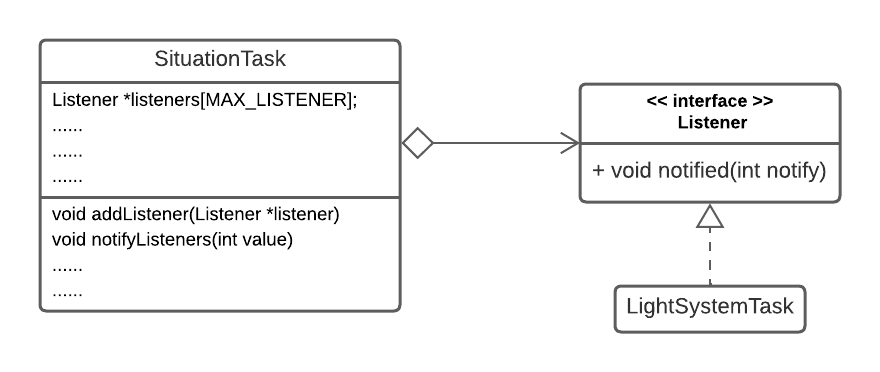
\includegraphics[width=13cm]{Observer.png}
    \caption{Rappresentazione UML del Pattern Observer}
\end{figure}
\'E stato utilizzato questo design pattern per far comunicare i 2 task principali:
\begin{itemize}
    \item LightSystemTask
    \item SituationTask
\end{itemize}

\par
Il LightSystemTask deve ricevere le  rilevazioni dal sonar, che è un componente del SituationTask.

\par
Grazie al Design Pattern Observer, ogni volta che il sonar rileva il livello dell'acqua, viene inviata una notifica al LightSystemTask, responsabile del funzionamento del sistema di Smart Light.

\par
Infatti come riportano le specifiche, se il livello dell'acqua è superiore ad una certa soglia, quindi se siamo in stato di allarme, il LightSystemTask deve spegnersi.
\par
Per L'implementazione di questo Design Pattern è stata creata un'interfaccia Listener, che definisce il metodo notified, poi implementato dal LightSystemTask.
\par
La classe SituationTask è composta da un array di Listener: in questo modo, ogni volta che viene effettuato un rilevamento dal sonar, viene richiamata la funzione notified su ogni elemento presente nell'array di listener per informarli dello stato del ponte.

\subsection{Strategy Design Pattern}
\begin{figure}[H]
    \centering
    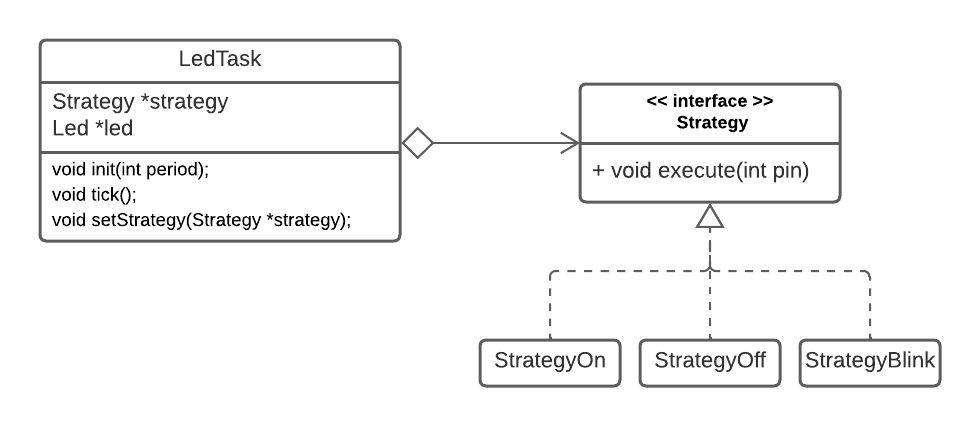
\includegraphics[width=13cm]{Strategy.png}
    \caption{Rappresentazione UML del pattern strategy}
\end{figure}
\par
\'E stato utilizzato Strategy design pattern per aggiungere funzionalità in modo semplice ai led.
\par
\'E stata quindi creata un'interfaccia Strategy, che definisce il metodo execute(), e le varie implementazioni: StrategyOn, StrategyOff, StrategyBlink, infine una classe chiamata LedTask.
\par 
La funzione tick() del LedTask, richiama la funzione execute() del componente Strategy, in questo modo, settando la Strategy per il LedTask, possiamo esprimere che funzionalità vogliamo utilizzare quando lo scheduler da la priorità al led in questione.

\chapter{Grafico}
\subsection{Descrizione}
\begin{figure}[H]
    \centering
    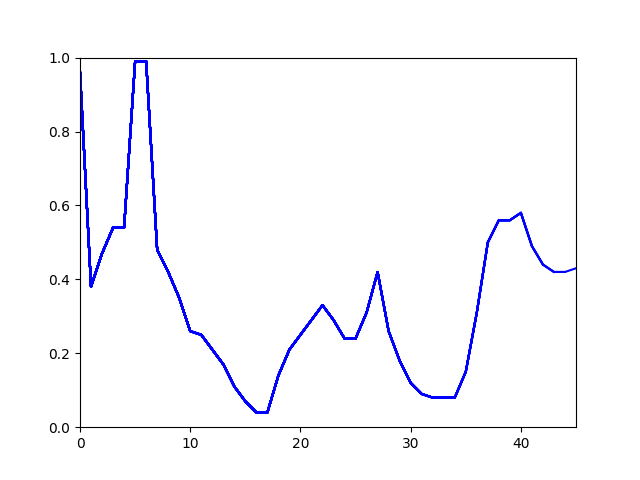
\includegraphics[width=10cm]{graph.png}
    \caption{Il grafico che rappresenta il livello dell'acqua nel tempo}
\end{figure}
\par
Lo script di Python denominato graph.py ha il compito di mostrare a schermo un grafico dinamico rappresentante il cambiamento del livello dell'acqua rilevato dal sonar nel tempo. Per ottenere questo risultato sono state usate varie librerie di Python, tra cui le più importanti sono  matplotlib, che permette di disegnare il grafico in poche semplici righe di codice, e Pyserial che permette allo script di leggere l'output nella console seriale di Arduino, estraendone i dati da inserire nel grafico.

\chapter {Tinkercad}
\begin{figure}[H]
    \centering
    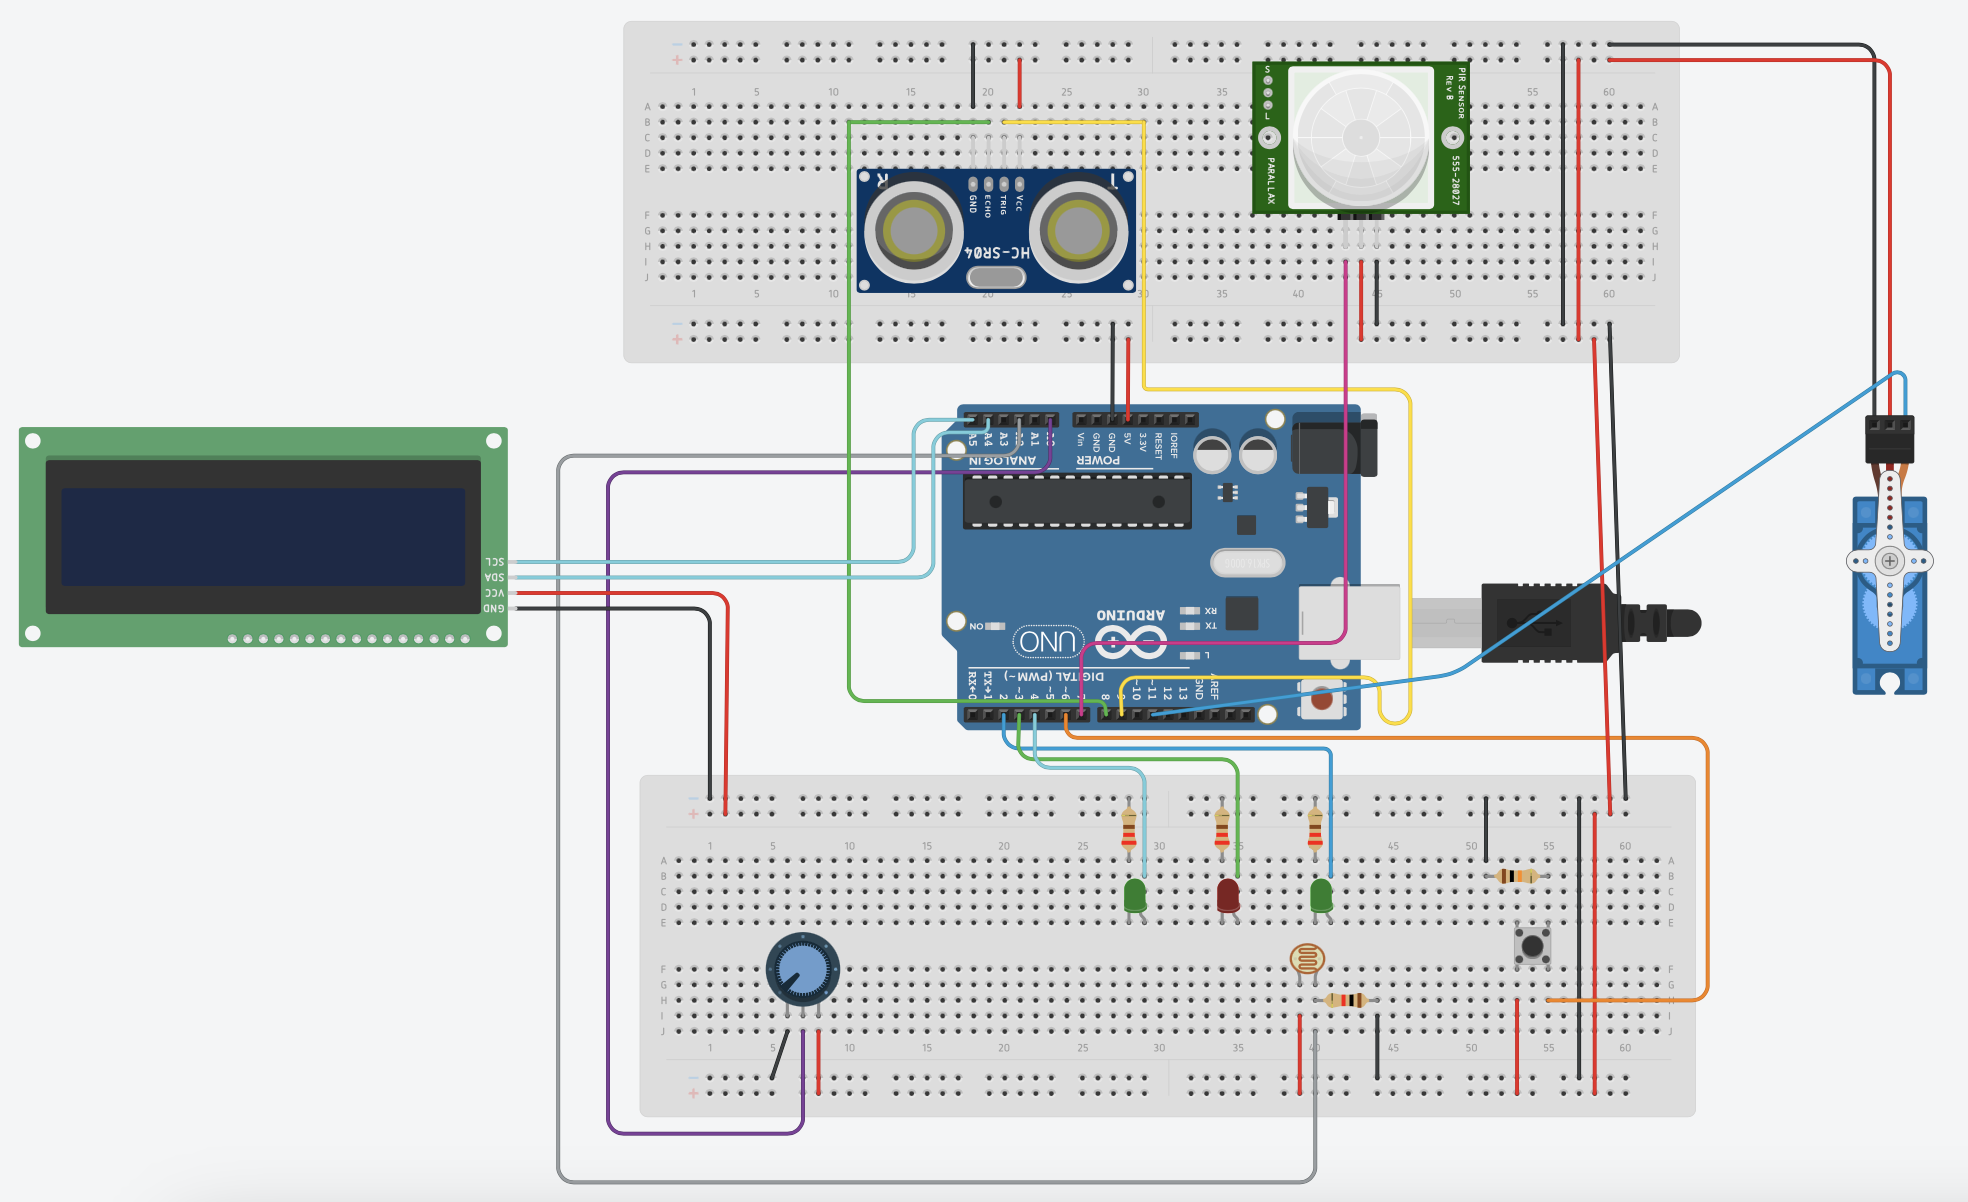
\includegraphics[width=15cm]{Screenshot 2022-11-30 alle 23.05.18.png}
    \caption{Tinkercad}
\end{figure}
\end{document}
